\documentclass[12pt]{article}
\usepackage{amsmath, amssymb, graphicx, hyperref}
\usepackage{indentfirst}
\usepackage{xcolor}
\usepackage{times}
\usepackage[sorting=none]{biblatex}
\usepackage[font=small,skip=0pt]{caption}
\usepackage{titlesec}
\usepackage[top=2.54cm, bottom=2.54cm, left=2.54cm, right=2.54cm]{geometry}
\bibliography{refs}
\date{\today}

\begin{document}
% TITLE PAGE
\begin{titlepage}
    \begin{figure}
        
\includegraphics[width=5cm, height=5cm]{logo.png}
        \centering
    \end{figure}
    \begin{center}
        \textbf{\Large{Department of Physics, IIT Delhi}}\\
        \vspace*{1cm}
        \textbf{\Large{Course Code : PYL655}}\\
        \vspace*{0.2cm}
        \textbf{\Large {Semester - II, 2022-23}}\\
        \vspace*{1cm}
        \textbf{\LARGE{Laser Physics Term Paper}}\\
        \vspace*{1cm}
        \textbf{\Large {Harikesh Kushwaha (2021PHS7181)}}\\
        \vspace*{1cm}
        \textbf{\Large {Course Coordinator: Prof. M. R. Shenoy}}\\
        \vspace*{1cm}
    \end{center}
    \begin{flushleft}
        \underline{\textbf{\LARGE{Term Paper Topic}}}\\
        \Large{\textbf{Ray Transfer Matrix Approach}: Write a suitable algorithm and program for ray tracing in a spherical mirror resonator. See that for large number of rays, the ray diagram has the same appearance as that of a Gaussian beam.}
    \end{flushleft}
\end{titlepage}
\newpage
% INTRODUCTION
\section*{Introduction}
Ray tracing with the ray transfer matrix approach is a simple yet powerful tool to study the properties of an optical system. In this approach, rays are traced by use of matrices. In this paper, we will discuss the same in some detail. In the first section, we'll start by giving a brief introduction to the ray transfer matrix approach, the ray transfer matrix (RTM) itself, the assumptions underlying them, and how they are so powerful. In the second section, we'll calculate the RTM of some simple systems and then use it to create the RTM of the spherical mirror resonator (SMR). The third section will give some details about the algorithm which has been developed to trace the rays in an SMR using {\color{cyan}Matplotlib} and {\color{cyan}NumPy}. The fourth section has the results obtained by the algorithm and we will see that for a large number of rays, the ray diagram has the same appearance as that of a Gaussian beam.

\section{Ray Transfer Matrix Analysis}
Ray transfer matrix analysis is a way to perform ray tracing. In this method, each optical element is described as a \(2\times 2\) matrix. The incoming light ray is described by a column vector. The product of the matrix and the vector gives the outgoing ray. The product of the matrices of all the optical elements gives the overall transformation of the incoming ray. This method is used to analyze the propagation of light through optical systems, such as lenses and mirrors. It is also used to analyze the propagation of light through optical fibers.\cite{wikipedia}\cite{photonics}

This technique is derived using the paraxial approximation, which assumes that all the ray directions are at small angles \(\theta\) such that the following approximation holds:
\begin{align}
    \label{eq:paraxial}
    \begin{split}
        \sin \theta &\approx \theta \\
        \tan \theta &\approx \theta
    \end{split}
\end{align}
\subsection{Ray Transfer Matrix}
The \(2\times 2\) matrix used to trace the rays is called the ray transfer matrix. It is a matrix that describes how an incident light ray is transformed as it passes through an optical system, such as a lens or a mirror. The matrix is usually denoted as \(\mathbf{M}\) and is written as:
\begin{align}
    \label{eq:rtm}
    \mathbf{M} = \begin{bmatrix}
                     A & B \\
                     C & D
                 \end{bmatrix}
\end{align}

As the elements of the matrix are \(A\), \(B\), \(C\) and \(D\), the matrix is also called the ABCD matrix. The elements of the matrix are determined by the optical properties of the system.

\subsection{The Incoming Ray}
The incoming ray is described by a column vector \(\mathbf{r}\):
\begin{align}
    \label{eq:incoming}
    \mathbf{r} = \begin{bmatrix}
                     y \\
                     \theta
                 \end{bmatrix}
\end{align}
where \(y\) is the distance from the optical axis and \(\theta\) is the angle of the ray with respect to the optical axis.

The RTM approach then states that for any optical system with RTM \(\mathbf{M}\), if the incident ray is \(\mathbf{r_i}\) then the output ray \(\mathbf{r_f}\) will be:

\begin{align}
    \label{eq:rtm-transformation}
    \begin{split}
        \mathbf{r_f}    & =\mathbf{M}\mathbf{r_i}      \\
        \begin{bmatrix}
            y_f \\
            \theta_f
        \end{bmatrix} & = \begin{bmatrix}
            A & B \\
            C & D
        \end{bmatrix} \begin{bmatrix}
            y_i \\
            \theta_i
        \end{bmatrix}\end{split}
\end{align}

The elements of the matrix \(A\), \(B\), \(C\) and \(D\) are determined by the properties of the optical system.

\begin{figure}[h]
    \centering
    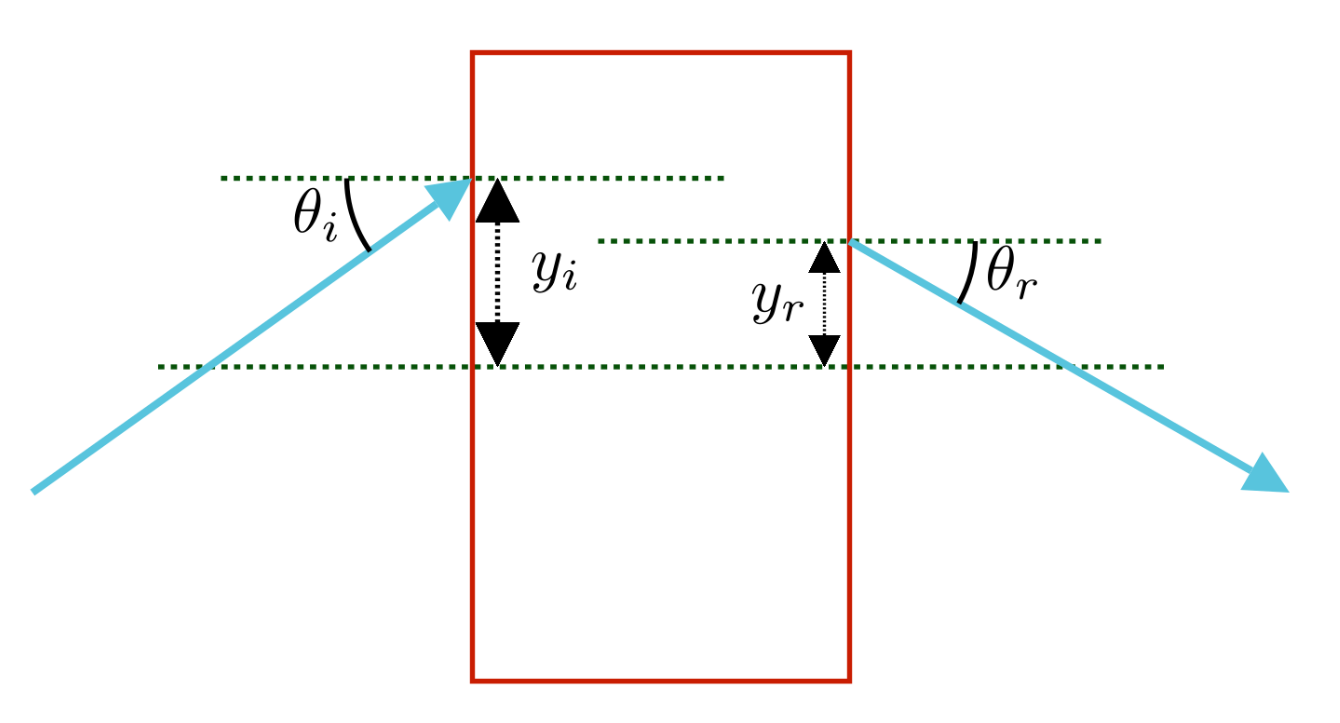
\includegraphics[width=0.75\textwidth]{images/box_c.png}
    \caption{A picture representing the incoming and outgoing rays (In blue arrows) through an optical system (depicted as a red rectangle). The input and output rays can be related by the equation \ref{eq:rtm-transformation}.\\ \textit{All the pictures in the paper are created by the author using {\color{cyan}manim}}\cite{manim}.}
    \label{fig:rtm-box}
\end{figure}
\subsection{Advantages of the RTM Approach}

The beauty of the RTM approach is that it does not matter what the optical system is, as long as we know the RTM for that system, we can do the ray tracing. Furthermore, if the system consists of a number of different optical elements, with different RTMs, the RTM of the complete system is just the multiplication of the whole system. For example, if there are four optical elements (as we will see in the case of the optical resonator) in the whole system with RTMs given by \(\mathbf{M_1}\), \(\mathbf{M_2}\), \(\mathbf{M_2}\) and \(\mathbf{M_4}\), the RTM of the system is:
\begin{equation*}
    \mathbf{M} = \mathbf{M_4}\mathbf{M_3}\mathbf{M_2}\mathbf{M_1}
\end{equation*}

This makes ray tracing very straightforward. Next, we'll consider the sign conventions used while calculating the RTM and tracing the rays.

\subsection{Sign Conventions}
\begin{figure}[h]
    \centering
    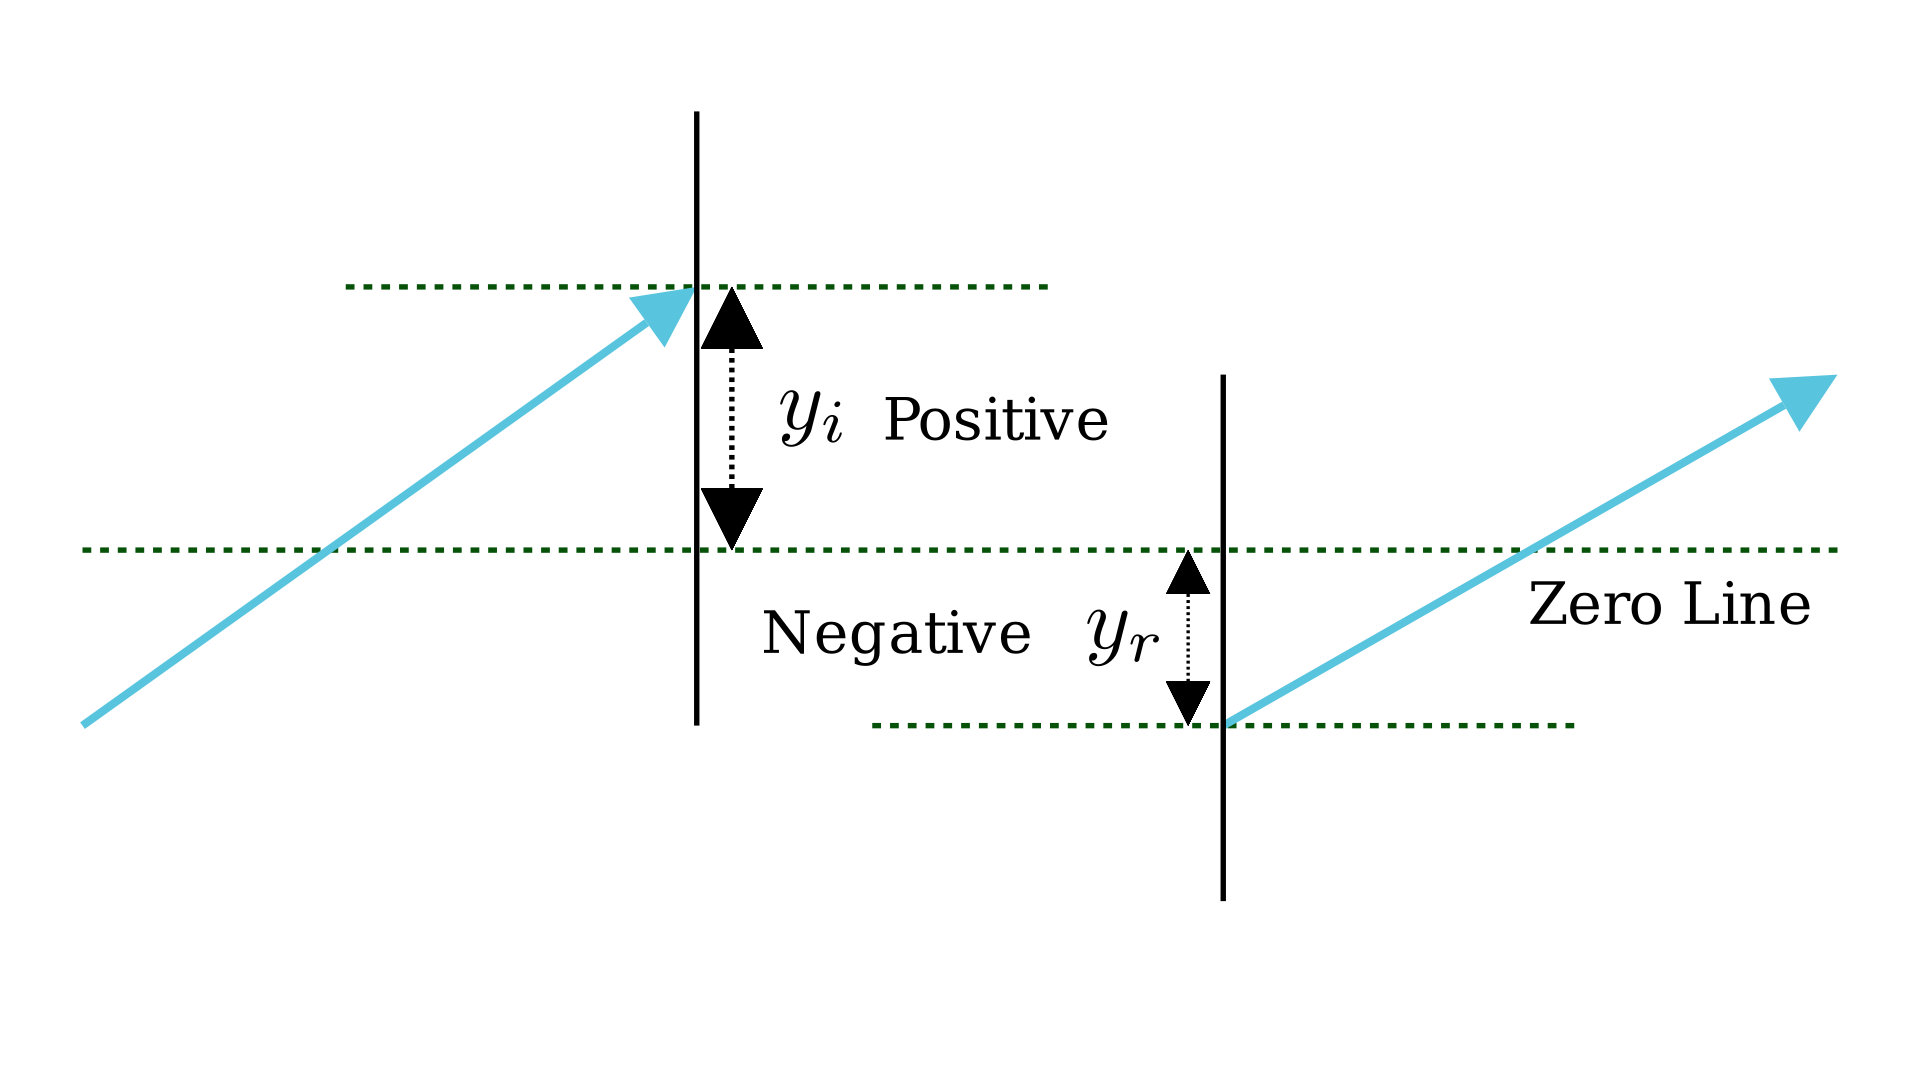
\includegraphics[width=0.7\textwidth]{images/sc_y_2.png}
    \caption{If the height is above the zero line (the optical axis), the sign is positive else is negative.}
    \label{fig:sign-y}
\end{figure}
The ray tracing technique is based on two reference planes, called the input and output planes, each perpendicular to the optical axis of the system. The first coordinate defining a ray, the height, is measured on this plane with reference to the optical axis. The figure above shows the optical axis as the \textit{zero line}. Using this, the sign convention is:
\begin{enumerate}
    \item The height \(y\) is positive if the ray is above the optical axis and negative if the ray is below the optical axis.
    \item The angle \(\theta\) is positive if the ray is moving above the optical axis and negative if the ray is moving below the optical axis.
    \item The radius of curvature of a concave mirror is negative and that of a convex mirror is positive.
\end{enumerate}
\begin{figure}[h]
    \centering
    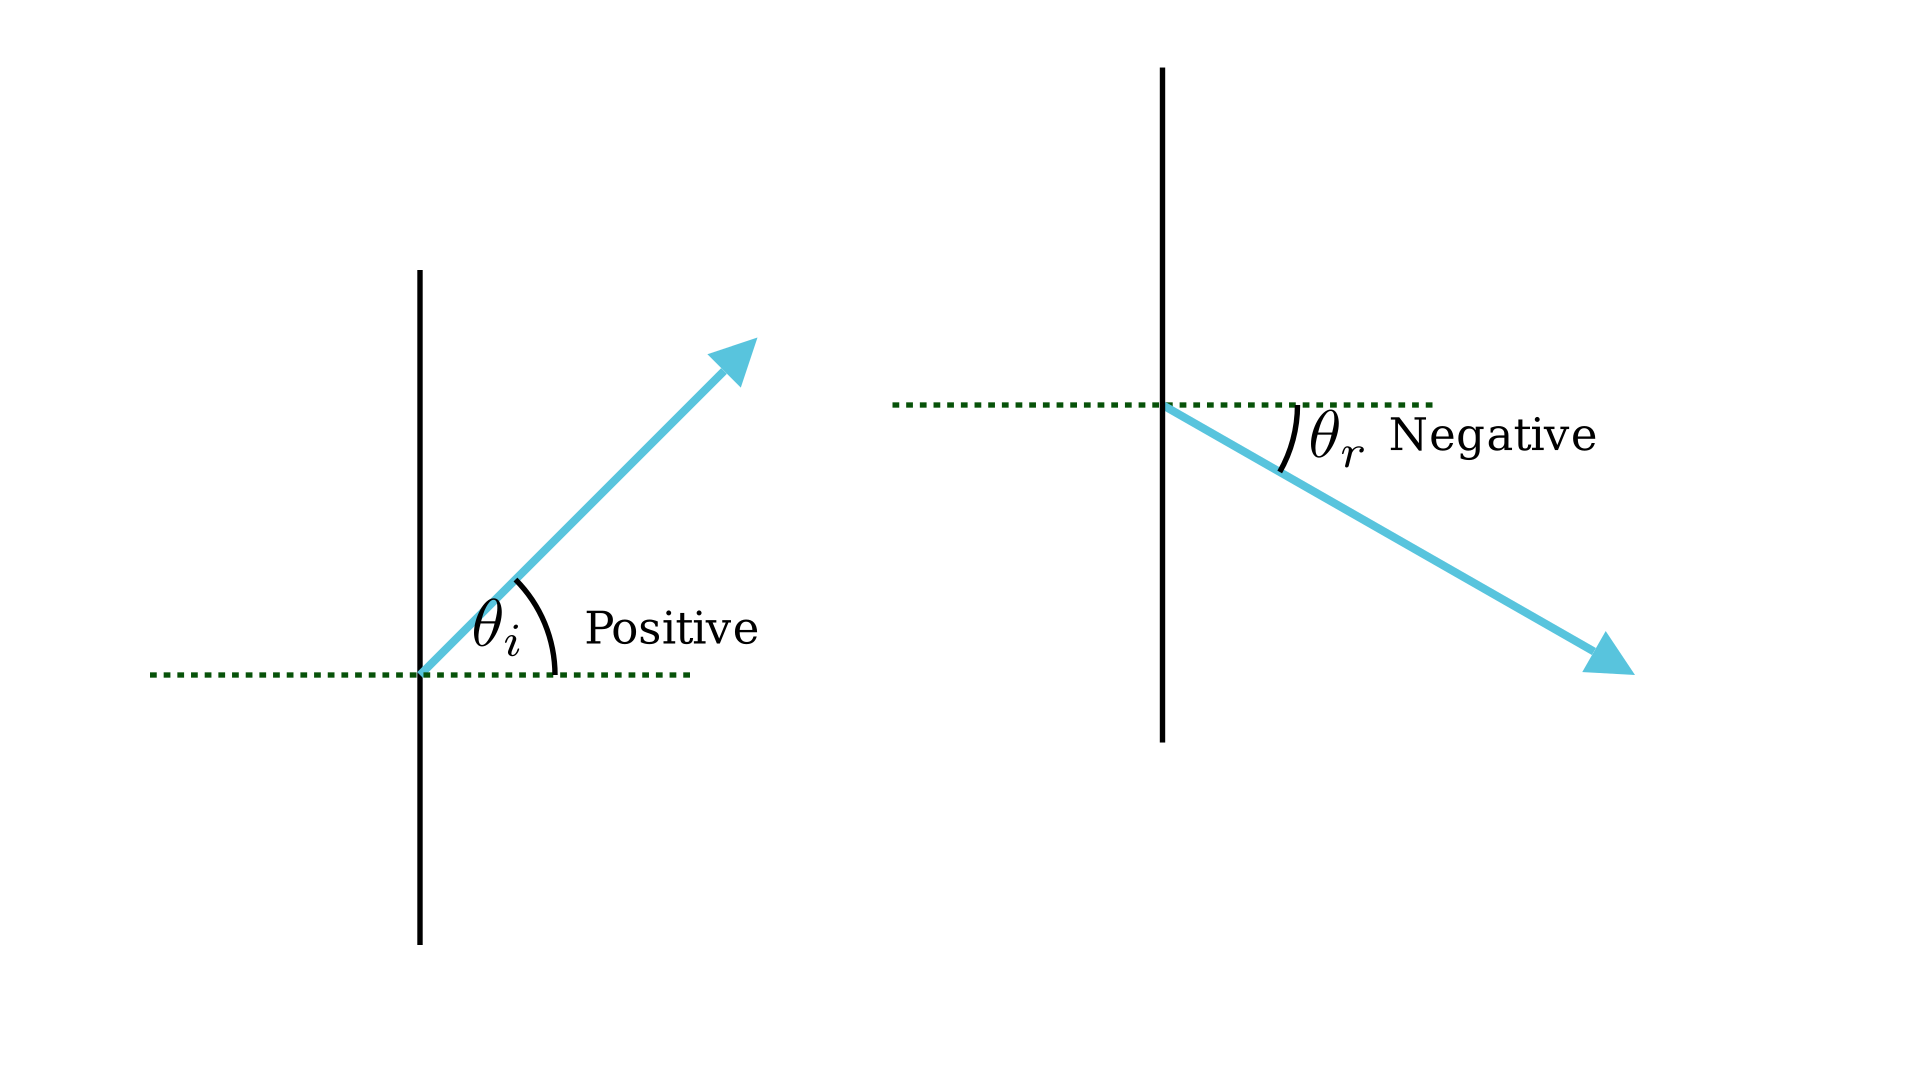
\includegraphics[width=0.7\textwidth]{images/sc_2.png}
    \caption{The angle \(\theta\) is positive if the ray is moving above the optical axis and negative if the ray is moving below the optical axis.}
    \label{fig:sign-theta}
\end{figure}

\section{RTM for Spherical Mirror Resonator}
\begin{figure}[h]
    \centering
    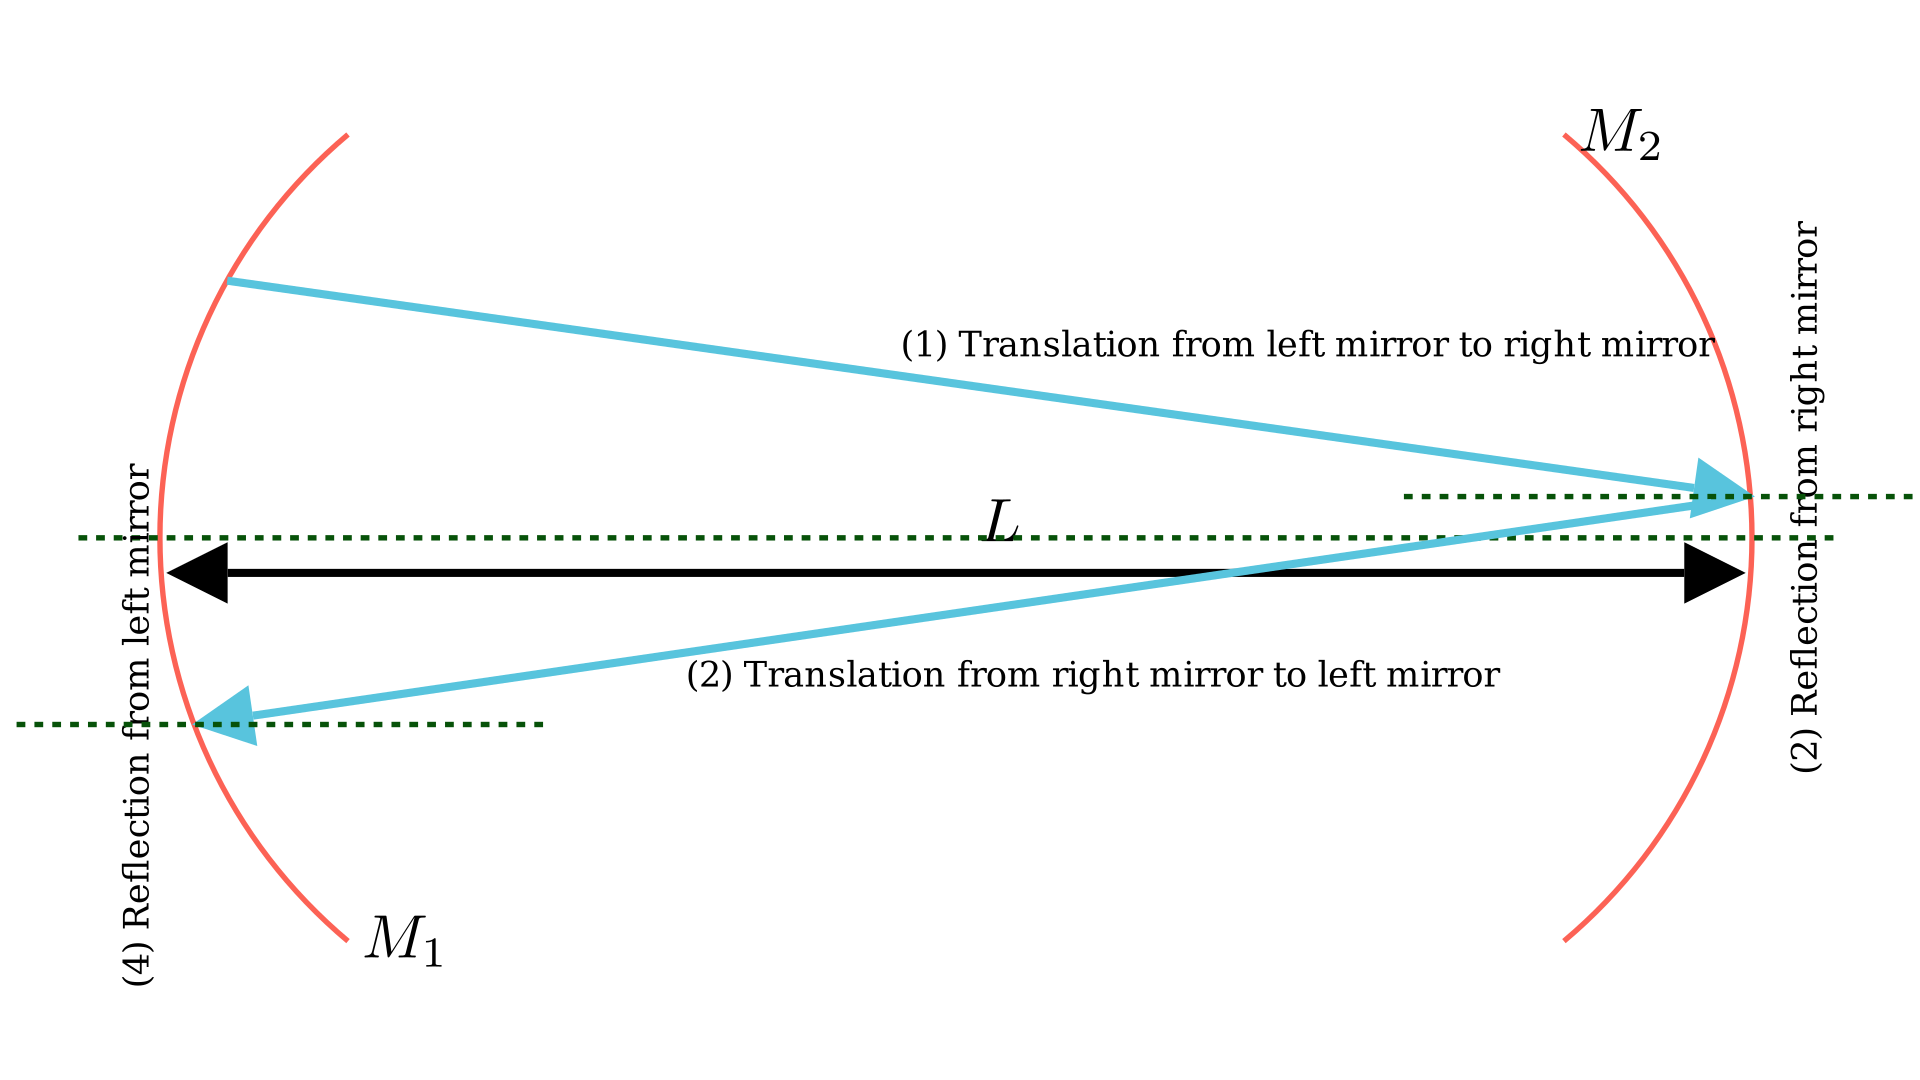
\includegraphics[width=0.9\textwidth]{images/round_trip.png}
    \caption{A round trip in an SMR consists of four different transformations.}
    \label{fig:round-trip}
\end{figure}

For ray tracing, we need to know the RTM of the SMR. In an SMR, the rays undergo four different transformations while going from the left mirror to the right mirror and back. These transformations are:
\begin{enumerate}
    \item Propagation through the resonator (from left to right), distance L
    \item Reflection from the left mirror \(M_2\)
    \item Propagation through the resonator (from right to left), distance L
    \item Reflection from the right mirror \(M_1\)
\end{enumerate}

So, we need to calculate the RTM for each of these transformations and then multiply them to get the RTM of the whole system.

\subsection{Propagation Through a Distance of L}
\begin{figure}[h]
    \centering
    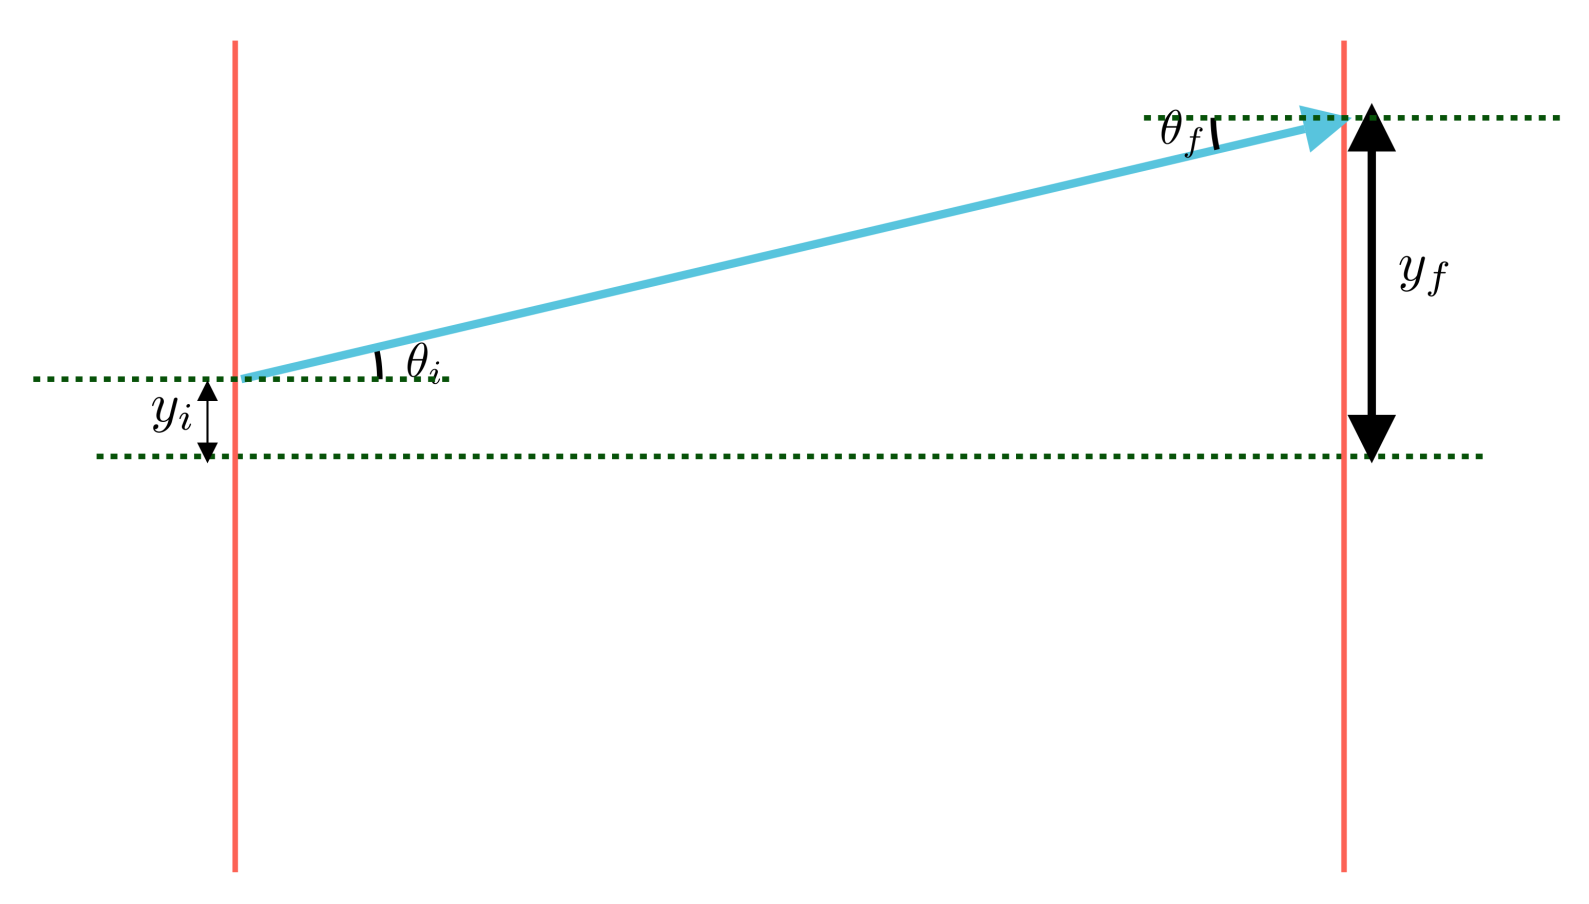
\includegraphics[width=0.7\textwidth]{images/translation.png}
    \caption{Propagation through a distance of L.}
    \label{fig:translation}
\end{figure}

We can see from Figure \ref{fig:translation} that during the propagation through a distance \(L\), the angles of the rays remain the same but the height changes. That is:
\begin{align}
    \begin{split}
        \theta_r & = \theta_f \\
        y_f & = L\tan\theta_r + y_i \approx L\theta_r + y_i
    \end{split}
\end{align}
This can be rewritten as:
\begin{align}
    \begin{split}
        \begin{bmatrix}
            y_f \\
            \theta_f
        \end{bmatrix} & = \begin{bmatrix}
            1 & L \\
            0 & 1
        \end{bmatrix} \begin{bmatrix}
            y_i \\
            \theta_i
        \end{bmatrix}
    \end{split}
\end{align}
So, the RTM for this transformation is:
\begin{align}
    \label{eq:translation}
    \begin{split}
        \mathbf{M} & = \begin{bmatrix}
            1 & L \\
            0 & 1
        \end{bmatrix}
    \end{split}
\end{align}

\subsection{Reflection from a Spherical Mirror}
\begin{figure}[h]
    \centering
    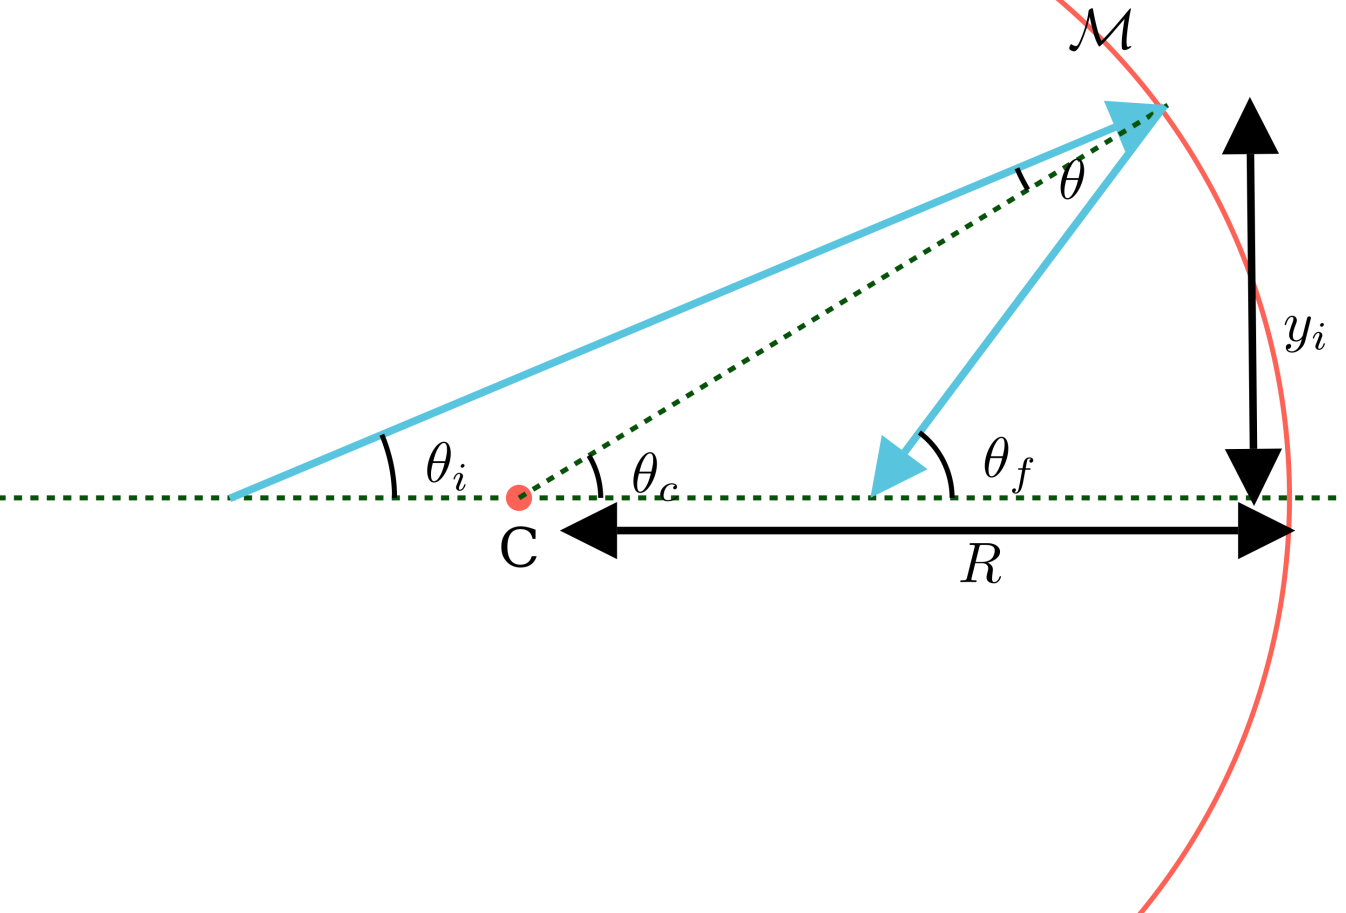
\includegraphics[width=0.7\textwidth]{images/reflection.png}
    \caption{Reflection from a spherical mirror.}
    \label{fig:reflection}
\end{figure}
For reflection from a spherical mirror, the height remains the same while the angle changes. So:
\begin{equation*}
    y_f = y_i
\end{equation*}
To determine the relation between the incoming and outgoing angles, we use Figure \ref{fig:reflection} above to write:
\begin{equation*}
    \theta_c = \theta_i + \theta
\end{equation*}
and
\begin{equation*}
    \theta_f = \theta_c + \theta
\end{equation*}
Subtracting these two gives:
\begin{equation}
    \label{eq:theta-f}
    \theta_f + \theta_i = 2\theta_c
\end{equation}
Using the paraxial approximation, we can write:
\begin{align}
    \begin{split}
        2\theta_c &\approx 2 \tan{\theta_c}\\
        & = -2\frac{y_i}{R} \quad \quad\text{(Using the sign convention)}\\
        \Rightarrow -\theta_f + \theta_i &= -2\frac{y_i}{R} \quad \quad\text{(Again, using the sign convention)}\\
        \theta_f &= \theta_i + \frac{2y_i}{R}
    \end{split}
\end{align}
This means that we can write:
\begin{align}
    \begin{split}
        \begin{bmatrix}
            y_f \\
            \theta_f
        \end{bmatrix} & = \begin{bmatrix}
            1           & 0 \\
            \frac{2}{R} & 1
        \end{bmatrix} \begin{bmatrix}
            y_i \\
            \theta_i
        \end{bmatrix}
    \end{split}
\end{align}

So, the RTM for this transformation is:
\begin{align}
    \label{eq:reflection}
    \begin{split}
        \mathbf{M} & = \begin{bmatrix}
            1           & 0 \\
            \frac{2}{R} & 1
        \end{bmatrix}
    \end{split}
\end{align}

\subsection{The RTM of the SMR}
Using the equations \ref{eq:translation}, \ref{eq:reflection} and the fact that the rays undergo four transformations, we can write the RTM of the SMR by multiplying these matrices. Assuming the radii of curvature of the left and right mirrors are \(R_1\) and \(R_2\) respectively, and the distance between the mirrors is \(L\), the RTM of the SMR is:
\begin{align}
    \label{fig:RTM-SMR}
    \begin{split}
        \mathbf{M} & = \begin{bmatrix}
            1             & 0 \\
            \frac{2}{R_1} & 1
        \end{bmatrix}
        \begin{bmatrix}
            1 & L \\
            0 & 1
        \end{bmatrix}
        \begin{bmatrix}
            1             & 0 \\
            \frac{2}{R_2} & 1
        \end{bmatrix}
        \begin{bmatrix}
            1 & L \\
            0 & 1
        \end{bmatrix}
    \end{split}
\end{align}

These are all the information needed to trace rays in the SMR.

\section{Ray Tracing}

The program to trace the rays in the SMR is written in Python. I've used {\color{cyan}Matplotlib}\cite{matplotlib} for the visualization and {\color{cyan}NumPy}\cite{numpy} for the matrix operations. All the codes and other related stuffs can be found in the \href{https://github.com/Hari31416/Laser-Term-Paper}{Github Repository}\cite{git-repo}.

\subsection{The Algorithm for Ray Tracing}
The algorithm for ray tracing is very straightforward and is as follows:
\begin{enumerate}
    \item Define the radius of curvature (ROC) of both the mirrors \(R_1 \& R_2\) and the distance between the mirrors \(L\).
    \item Use the equations \ref{eq:translation} and \ref{eq:reflection} to find the RTM for propagation \(M_P\), for the reflection from the left mirror \(M_{R_L}\) and for the reflection from the right mirror \(M_{R_R}\).
    \item Choose a starting point for the ray and the angle of incidence, say \(\mathbf{r_0} = [y_0, \theta_0]^T\). The ray will start from the left mirror.
    \item To determine the y-position of the ray when it reaches the right mirror, multiply \(\mathbf{r_0}\) with \(M_P\) and call it \(\mathbf{r_1}\). The y-coordinate of \(\mathbf{r_0}\) and the y-coordinate of \(\mathbf{r_1}\) can be used to draw a line that will give the path at which the ray travels from the left to right mirror. (Assuming that the x-coordinate of the mirrors are fixed, which is indeed the case.)
    \item Now, multiply \(\mathbf{r_1}\) with \(M_{R_R}\) (this will result in a change in the angle) and then again with \(M_P\). Call it \(\mathbf{r_2}\). This will give the y-position of the rays when it reaches the left mirror.
    \item Again, a line can be drawn using the y-positions of \(\mathbf{r_1}\) and \(\mathbf{r_2}\). This will depict the ray coming to the left mirror from the right mirror.
    \item Continue steps 4-6 by using the previous position vector as starting point. Stop once sufficient number of rays have been traced.
\end{enumerate}

\subsection{Some Detail About the Program}
This section gives some more detail about the program. The program is written using {\color{cyan}object-oriented programming} where we start by modeling the real-world objects in code. This makes the code very intuitive and easy to implement. The program uses two objects: {\color{cyan}Mirror} and {\color{cyan}Resonator}. Physically, a resonator is nothing but two mirrors separated by some distance. The {\color{cyan}Resonator} object is implemented likewise. A {\color{cyan}Resonator} can be instantiated by giving the radii of the two mirrors and the separation between them. Then the {\color{cyan}propogate()}  method can be called to trace the rays passing it the starting position and the number of rays to plot (This method uses the same algorithm outlined above to trace the rays.). Please refer to the \href{https://github.com/Hari31416/Laser-Term-Paper}{Github Repository} for the source code and for more detail on how the algorithm works.

\section{Results}
This section shows some ray diagrams of both stable and unstable resonators with ray tracing done by the program described above. We will see that for large number of rays, the ray diagram has the same appearance as that of a Gaussian beam.

The next two pages have ray diagrams for some resonators. First few diagrams are for stable resonators. Then we give one ray diagram for the unstable resonator. The resonator details and ray tracing details are given in the caption and in the diagram itself.
\begin{figure}[h]
    \centering
    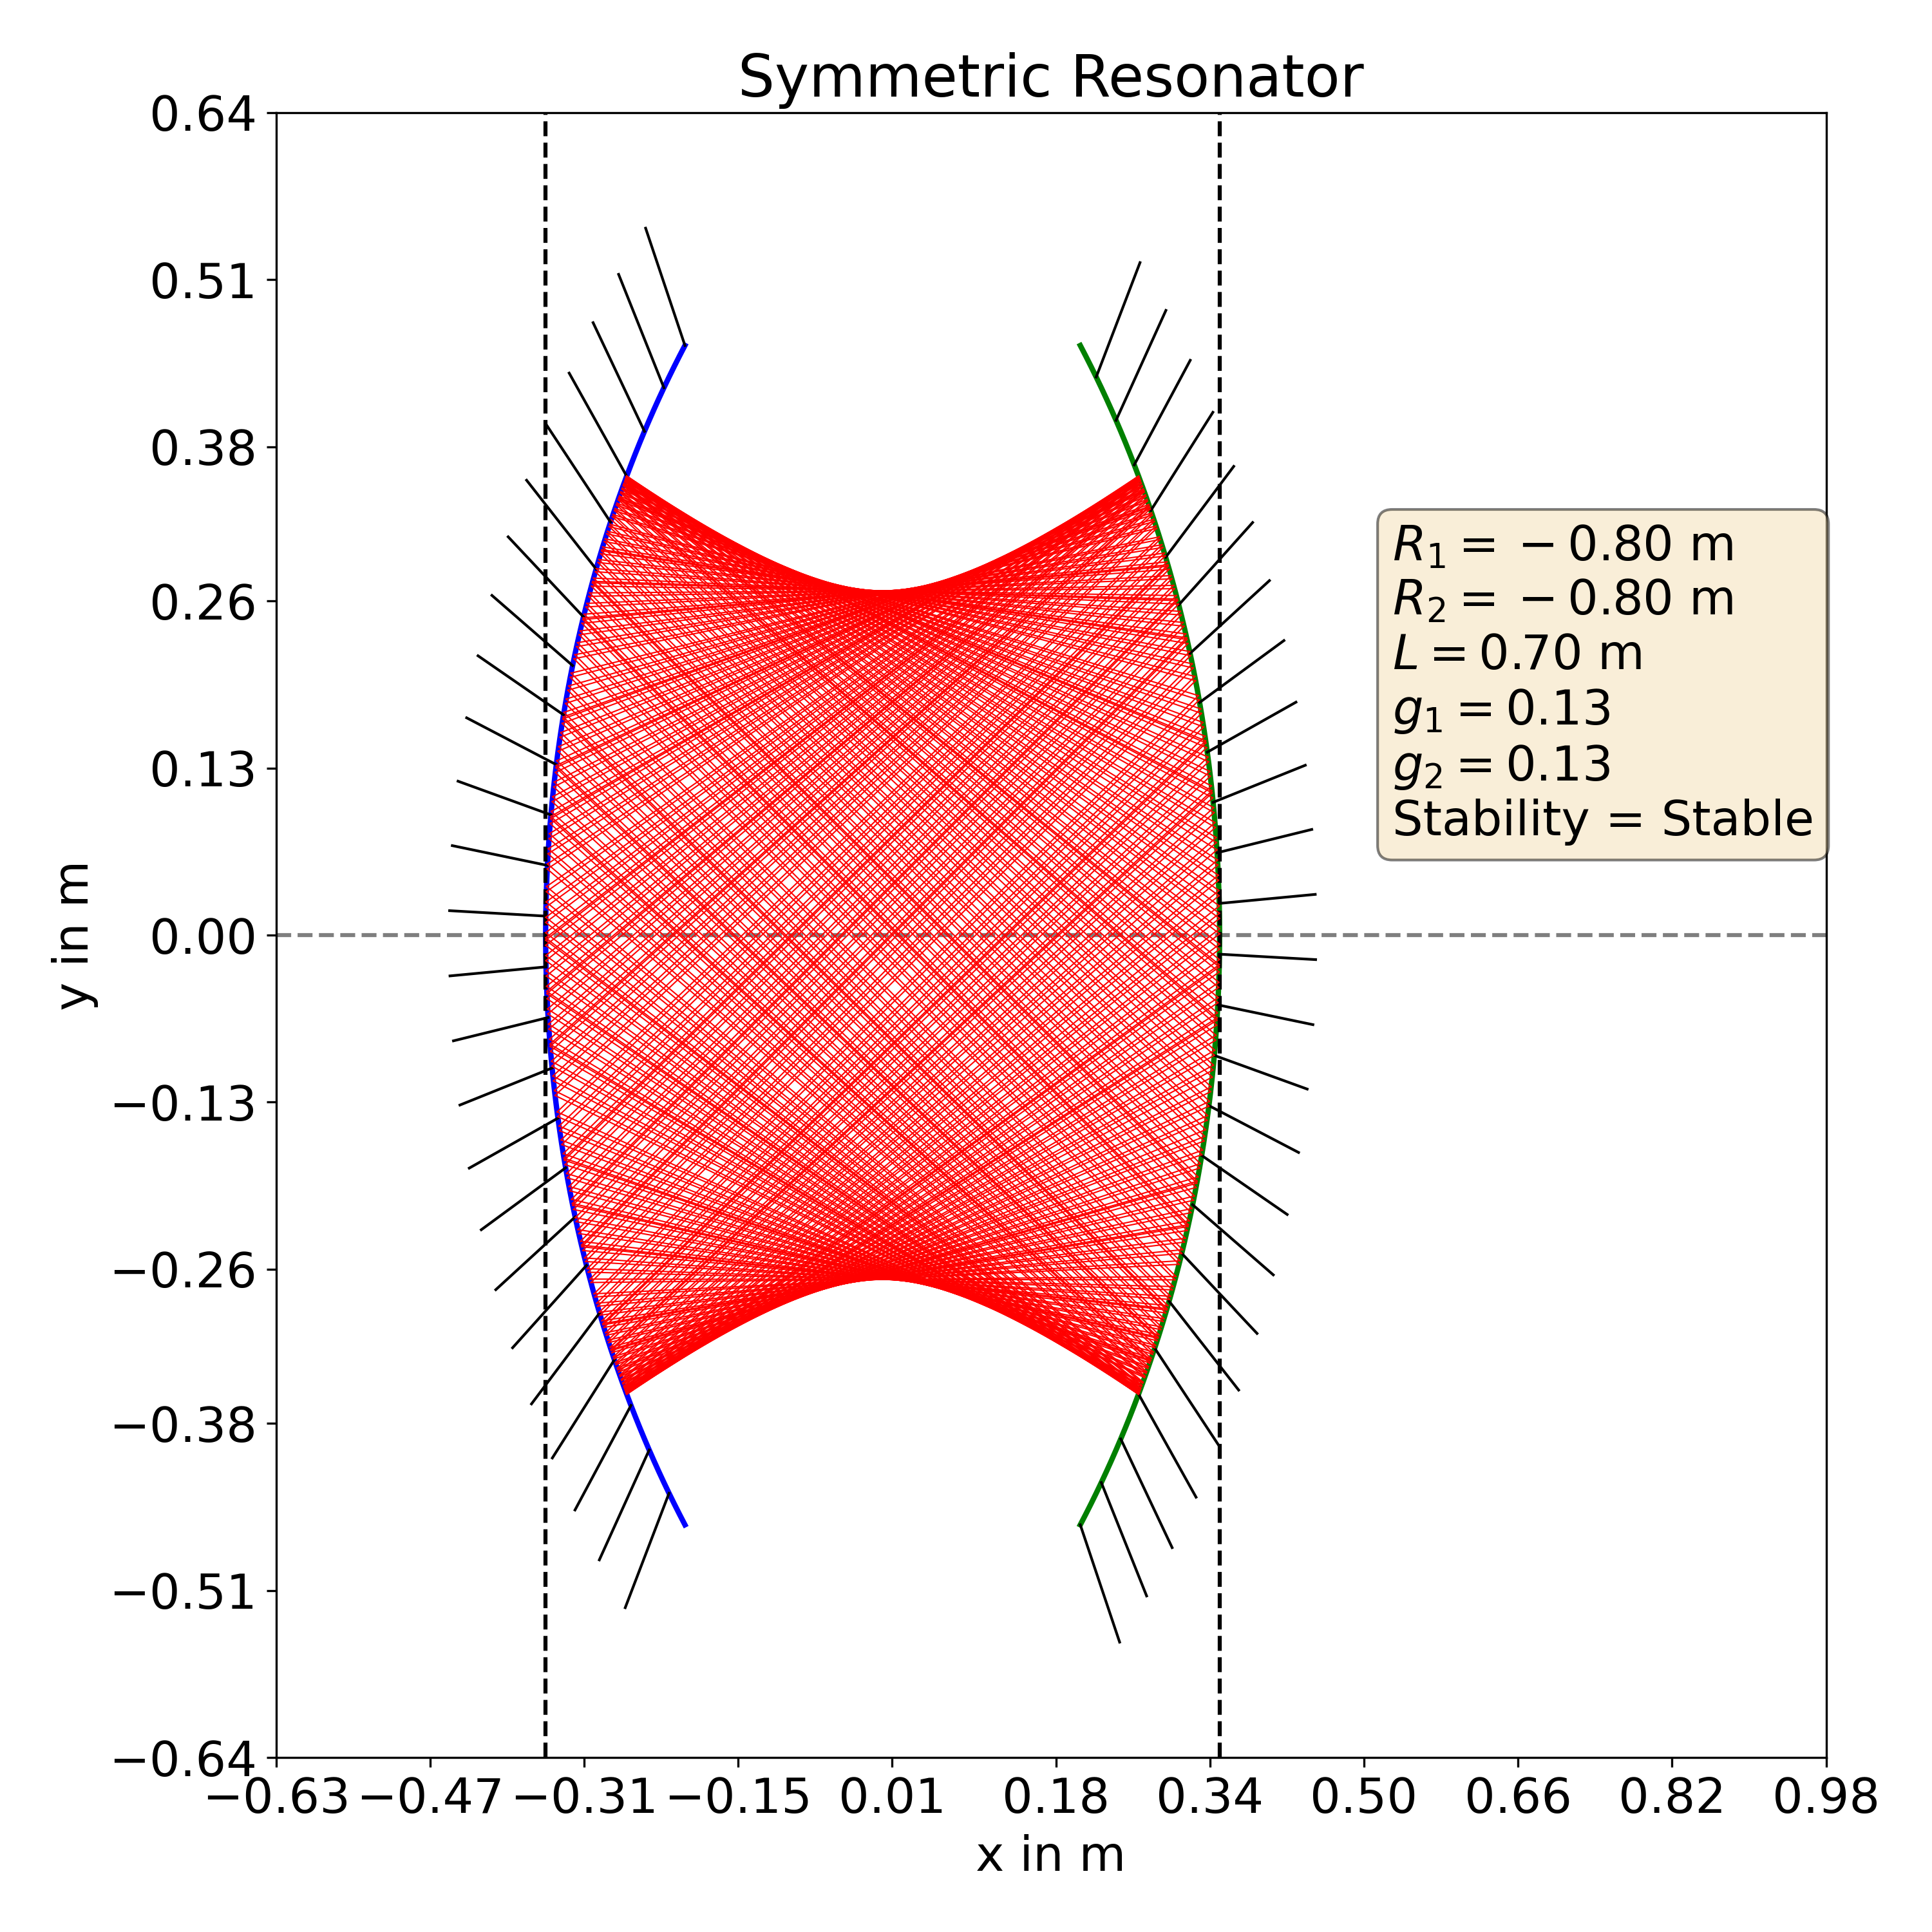
\includegraphics[width=0.6\textwidth]{images/symmetric.png}
    \caption{Ray diagram of a symmetric resonator. The metadata for the resonator is shown in the figure. The intial position is \([0.3, -0.1]^T\). 200 rays are traced. The Gaussian shape is readily observed.}
    \label{fig:symmetric}
\end{figure}

\begin{figure}
    \centering
    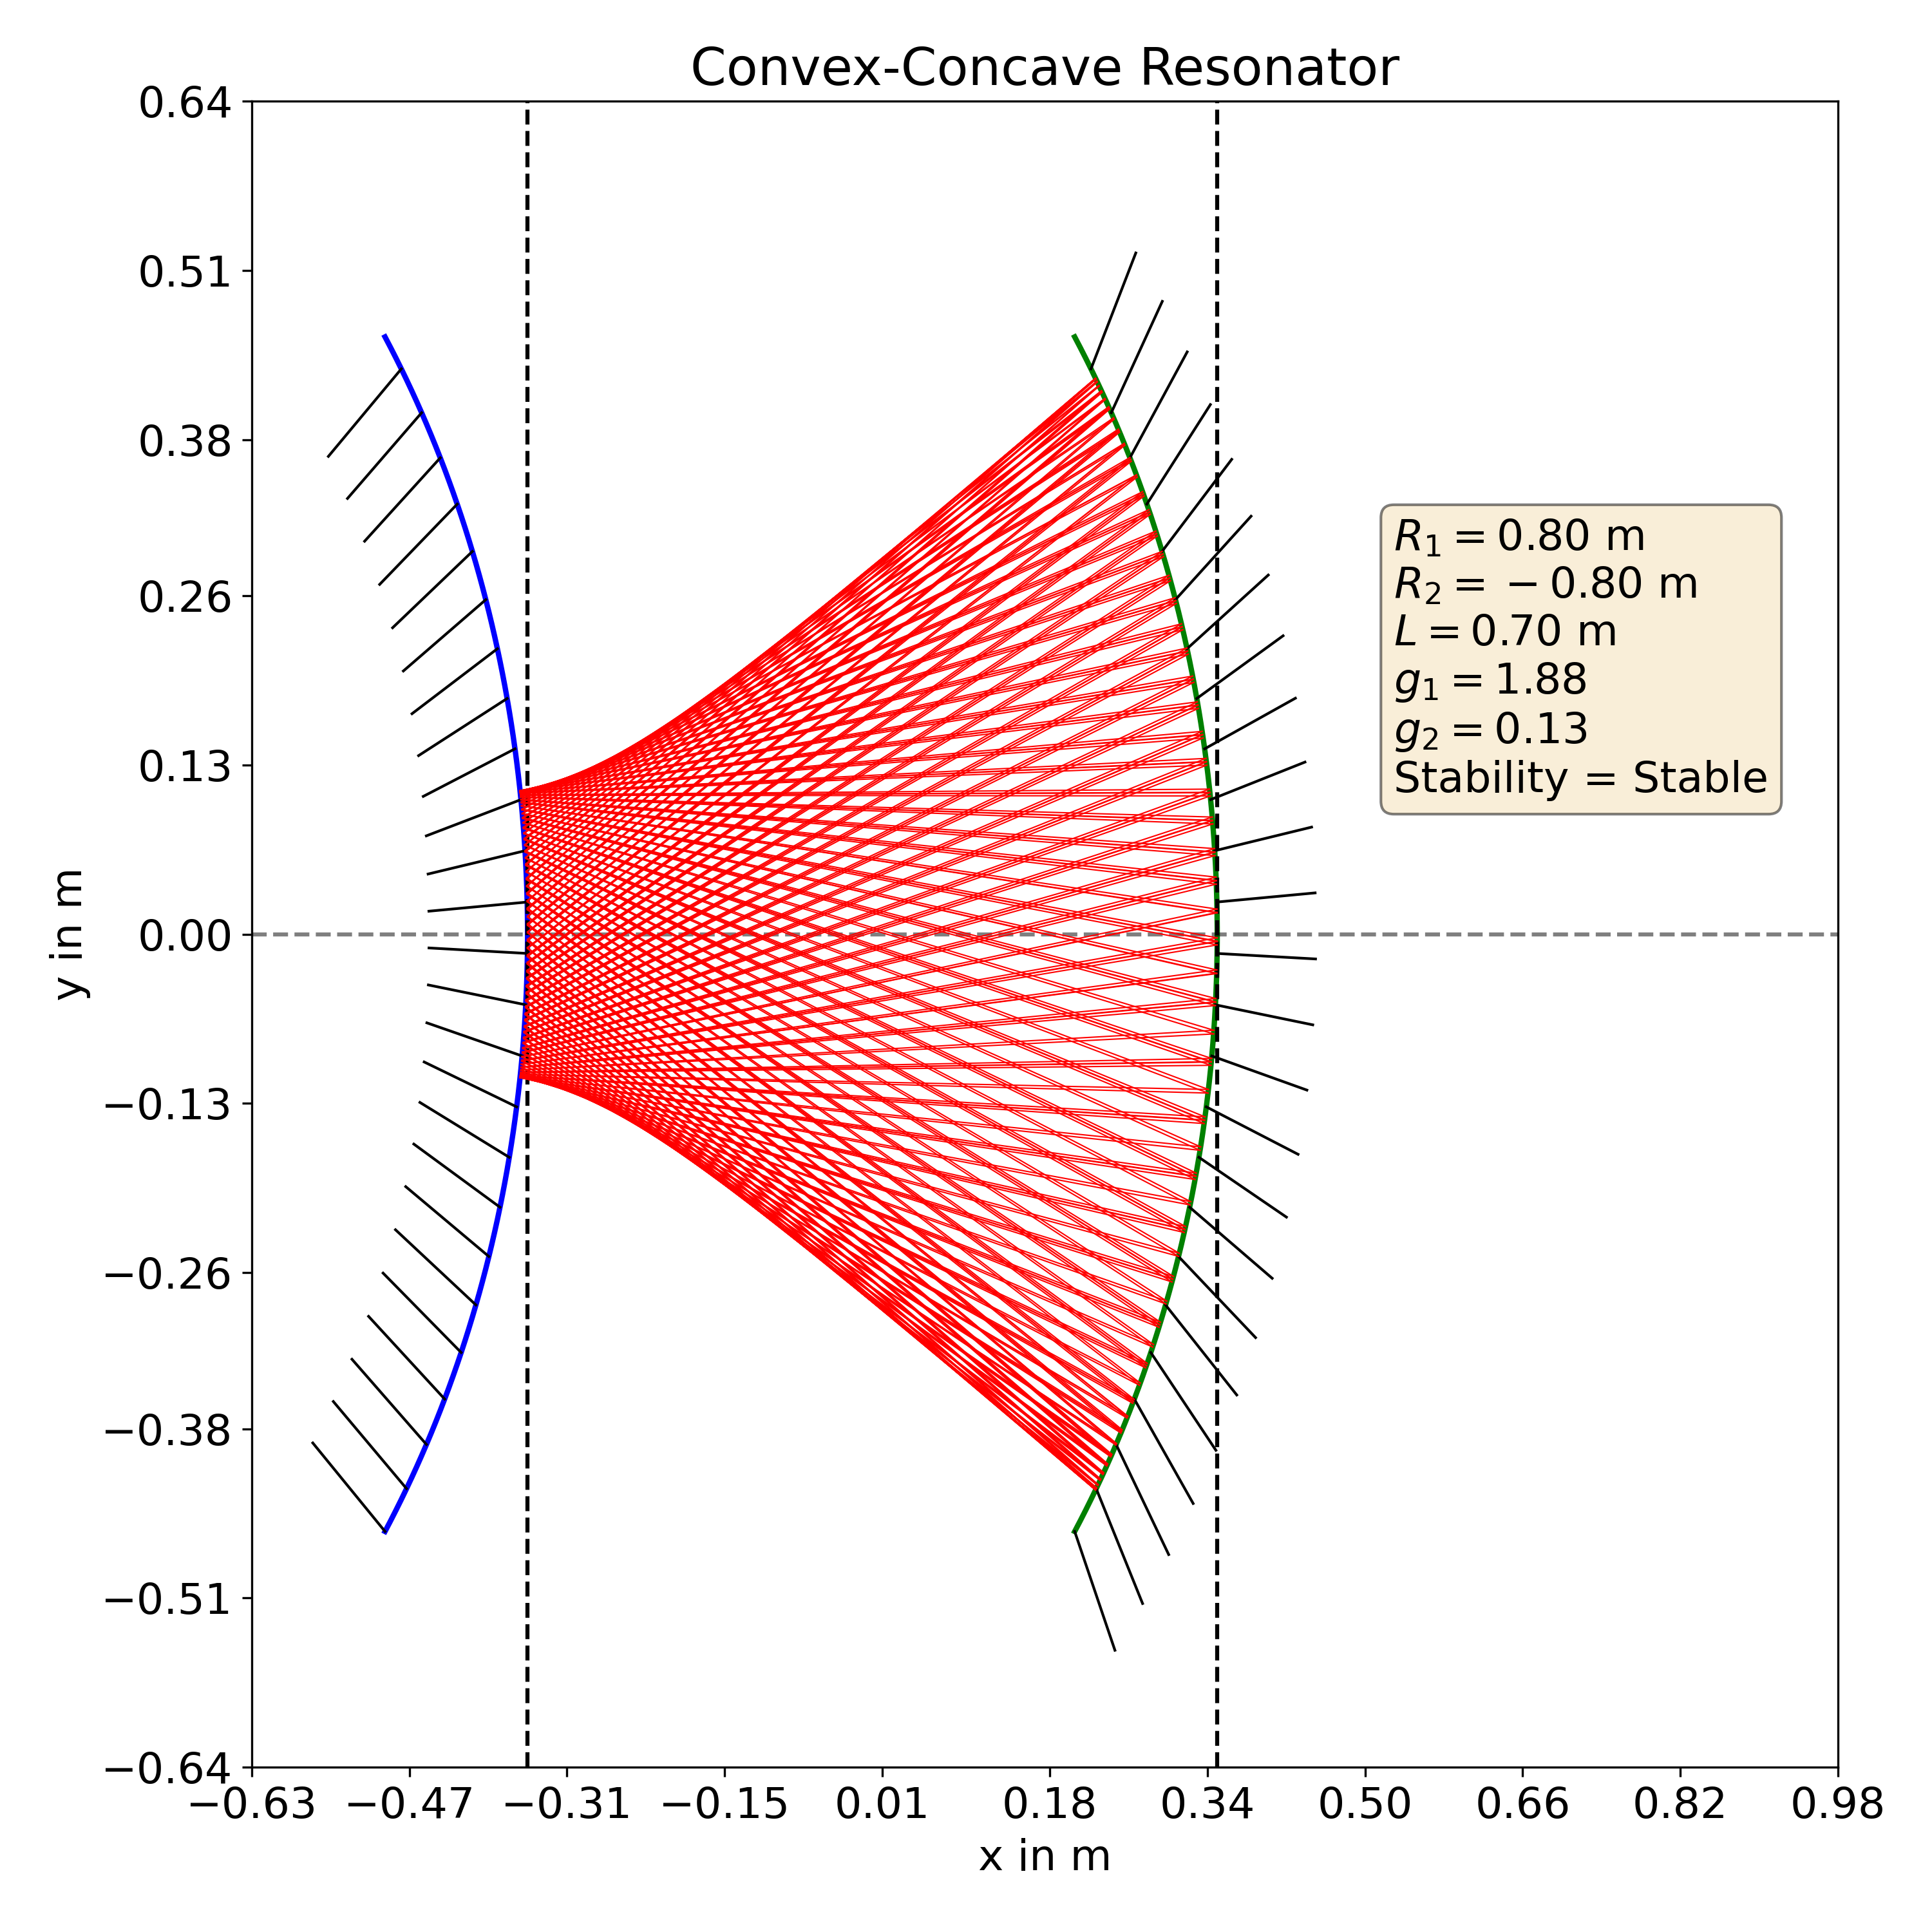
\includegraphics[width=0.6\textwidth]{images/cave_vex.png}
    \caption{Ray diagram of a resonator with one convex and once concave mirror. The metadata for the resonator is shown in the figure. The intial position is \([-0.1, 0.1]^T\). 200 rays are traced. Once again, the Gaussian shape can be seen.}
    \label{fig:cave-vex}
\end{figure}

\begin{figure}
    \centering
    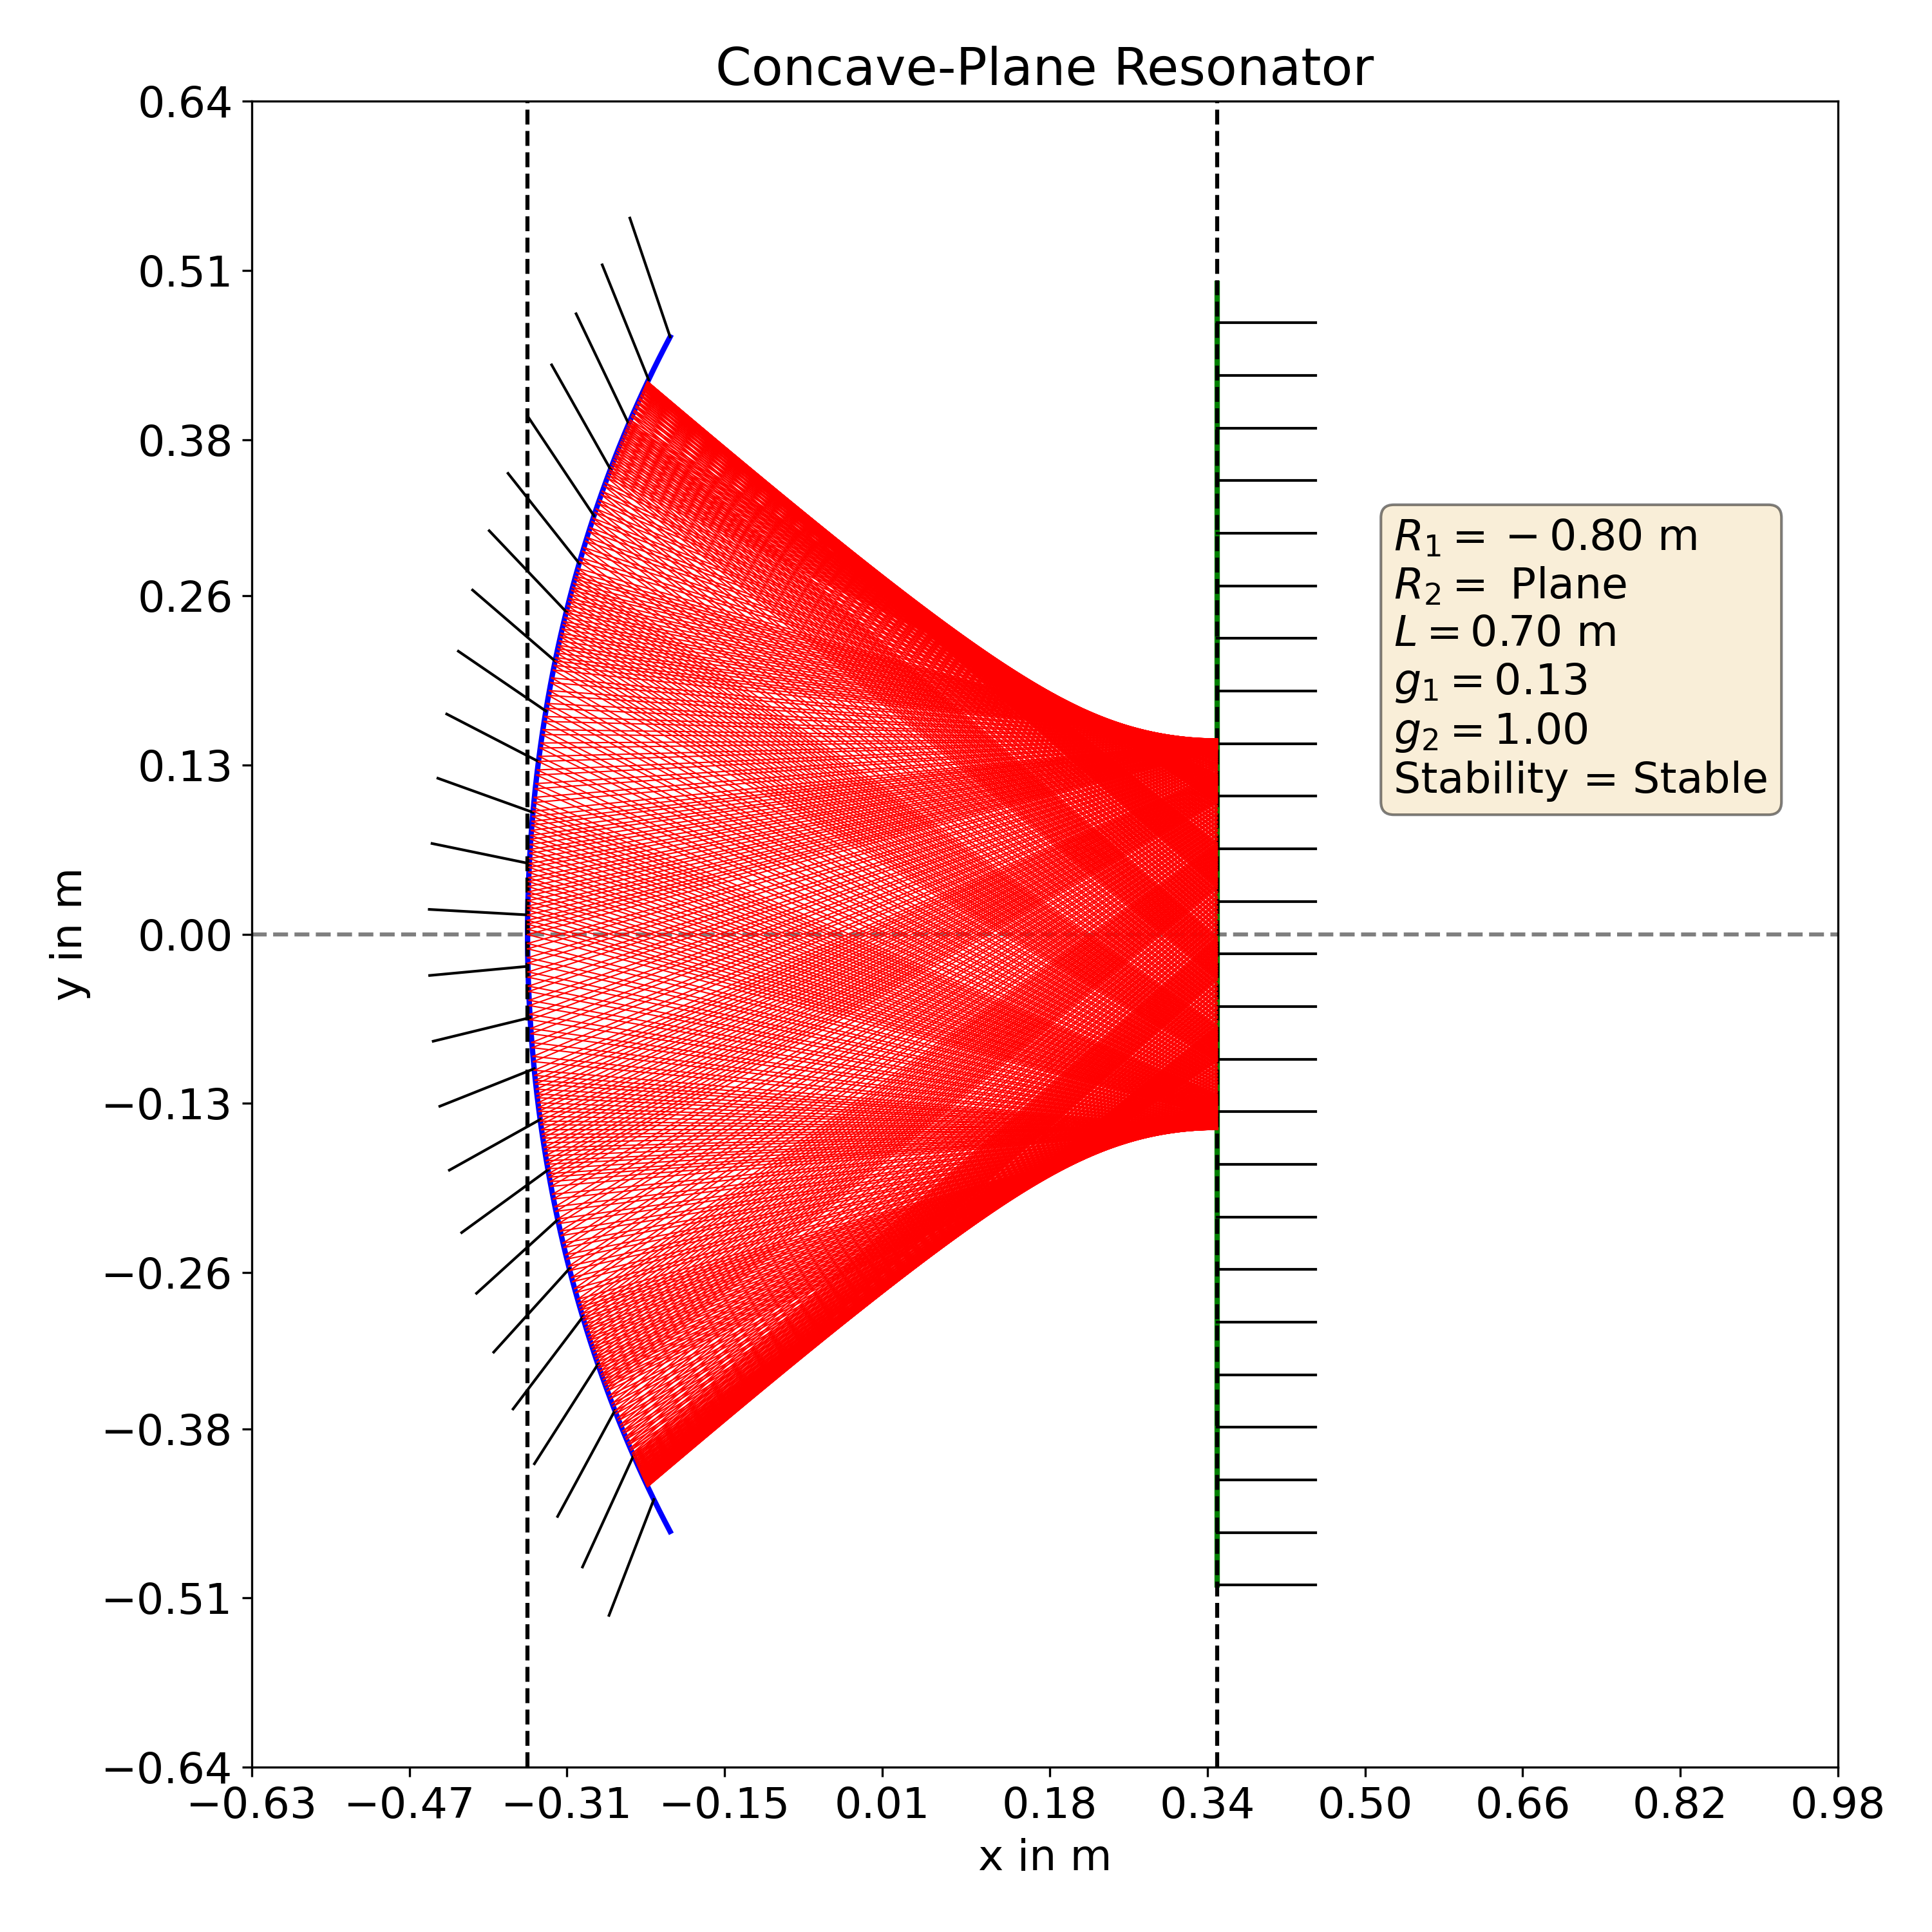
\includegraphics[width=0.55\textwidth]{images/plane_cave.png}
    \caption{A stable resonator can be created with plane mirror too, given that the second mirror is a concave one. The diagram shows such a resonator. The intial position is \([-0.15, 0]^T\). 300 rays are traced. The Gaussian shape can be see here too.}
    \label{fig:plane-vex}
\end{figure}

\begin{figure}
    \centering
    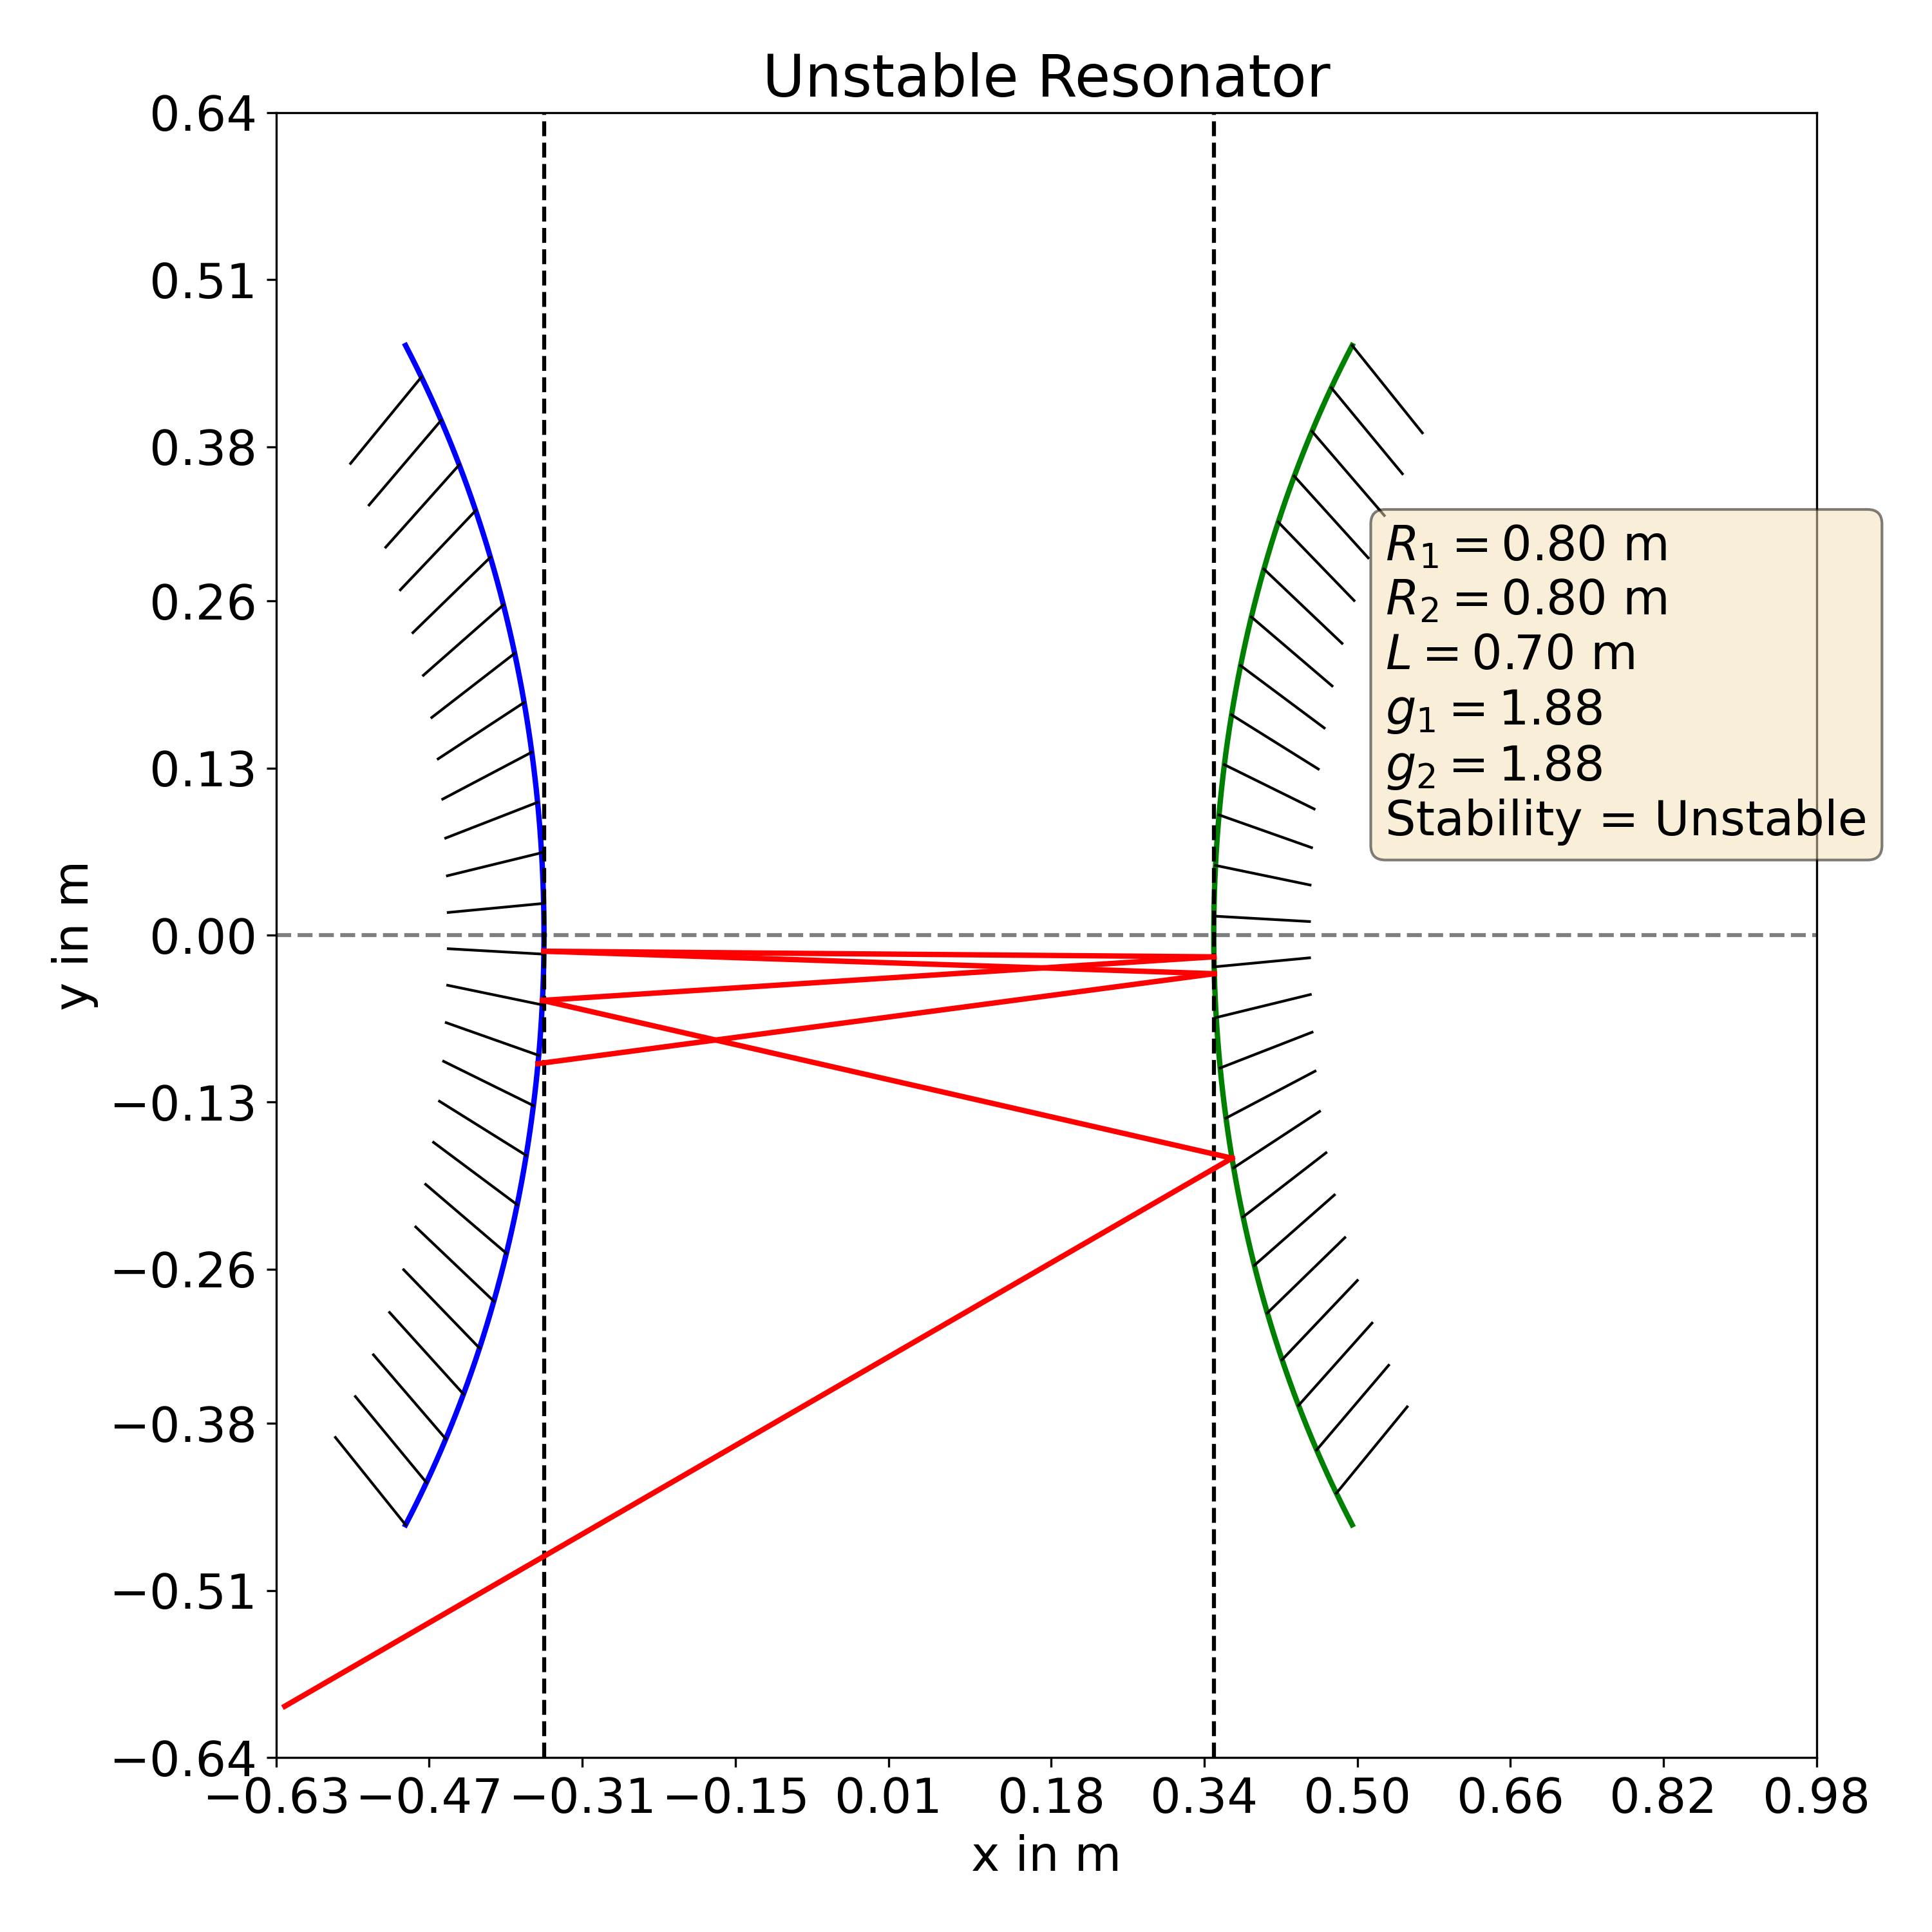
\includegraphics[width=0.55\textwidth]{images/unstable.png}
    \caption{Two convex mirrors can never form a stable resonator. The diagram shows such an unstable. The intial position is \([-0.1, 0.1]^T\). Less than 10 rays are inside the mirrors given in the figure.}
    \label{fig:unstable}
\end{figure}
\clearpage
\newpage
\section{Conclusion}
In this paper, we discussed how RTM can be used to trace rays in a SMR. We derived the RTM for the SMR and used it with {\color{cyan}Matplotlib} and {\color{cyan}NumPy} to write a program to trace the rays inside the given resonator. We plotted such ray diagrams for a number of stable resonators and found out that their shape resembles that of a Gaussian beam. We also saw ray diagram of an unstable resonator.
\printbibliography
% \end{changemargin}
\end{document}
\end{document}